\chapter{Introducción}

La publicación de datos abiertos por parte de ayuntamientos e instituciones públicas está cada vez más extendido y en un futuro se irá incrementando. Estos datos son completamente accesibles y reutilizables para cualquier fin que un usuario quiera darles, lo cual da mucha libertad a la hora de crear aplicaciones y dar valor a esa información.
Estos en su mayoría se encuentran en formato RDF, CSV u hojas de calculo. La publicación por parte de los ayuntamientos suele contener errores, incoherencias u otros problemas que impiden su correcta utilización. Es por ello que para su uso debe hacerse un análisis y determinar una estrategia y modelización de los mismos.


El trabajo consistirá en crear una aplicación que, a partir de los datos proporcionados por el ayuntamiento de Madrid, pueda hacer una valoración de las distintas calles acorde con la seguridad de las mismas para circular en bicicleta. Todo esto siguiendo los principios de Web Semántica y Linked Data que permita realizar un buen modelado de los datos, para su correcto funcionamiento y para una posible reutilización posterior.


Primero será necesario seleccionar los vocabularios con los que se va a trabajar. Para ello se reutilizarán los ya creados en la plataforma vocab.ciudadesabiertas.es \cite{ciudadesabiertas_catalogoVocabs} y se crearán nuevos a partir del portal de datos del ayuntamiento de Madrid \cite{datosabiertos_ayuntmadrid}. Se reutilizará el vocabulario de Callejero, definido en ciudadesabiertas\cite{ciudadesbiertas_callejero} y se propondrán las modificaciones pertinentes sugiriendo añadir nuevas propiedades.

Se han diseñado tres nuevos vocabularios a partir de los datasets proporcionados por el ayuntamiento de Madrid. El correspondiente a Accidentes, accesible en formato CSV y XLSX en la web \cite{datosMadrid_accidentesDeBicicleta}. Para este caso se han tenido en cuenta elementos de los accidentes de bicicletas, sin embargo se ha definido un vocabulario genérico para todo tipo de accidentes, ya que sería aplicable para otro tipo de vehículos. El correspondiente a Ciclocarriles, partiendo del dataset accesible en formato XLS y KML \cite{datosMadrid_ciclocarriles}. Y finalmente el correspondiente a Calles Tranquilas, accesible en formato XLS y KML en la dirección \cite{datosMadrid_callesTranquilas}. Para este último caso no se ha definido un nuevo vocabulario sino que se ha modificado el Callejero antes mencionado de forma que incorpore estas nuevas propiedades.


En este proyecto se va a desarrollar una aplicación que, a partir de estos datos y conociendo la ruta entre 2 puntos dentro de Madrid, se haga una valoración de todas las calles por las que transcurra y se pueda valorar las incidencias y propiedades de cada una de ellas, proporcionando una información detallada de los elementos que en ellas podemos encontrar y de los accidentes ocurridos. Para ello se hará uso de la API Directions de Google, de la cual se obtendrá la ruta entre las posiciones dadas por el usuario. Tras esto se obtendrán las vías correspondientes a cada uno de los puntos. Una vez se tengan las calles por las cuales el navegador GPS guiará al ciclista hasta su destino, se comprobará una a una su seguridad y se detallarán al usuario los Ciclocarriles que se encuentran en el recorrido, las calles que se consideran tranquilas y los accidentes ocurridos en el último año en las calles por las que va a circular. Por último se hará un cálculo aproximado de la seguridad del recorrido de modo que el usuario pueda valorar si realizarlo en bicicleta o no.


Para esta comprobación se hará uso de los datos mencionados antes. Para ello, se le asignará un identificador único a cada calle, el cual es proporcionado por el Callejero del ayuntamiento \cite{datosmadrid_callejero} y definido como se ha mencionado anteriormente en el portal ciudadesAbiertas. Este identificador ha sido asignado a los tres datasets, cuyos vocabularios han sido definidos en el contexto de este trabajo, y de esta forma es posible hacer una búsqueda rápida y concisa de cada calle por la que transitará la ruta, para así conocer mejor las características de ellas y determinar su seguridad.


Más adelante se detallarán los elementos de cada vocabulario utilizado en la aplicación. En términos generales, en la figura \ref{fig:esquemaTotalVocab} se muestran los elementos que se han definido y utilizado para esta aplicación y de forma genérica el enlazado entre ellos.


\clearpage
\begin{figure}[h]
  \centering
  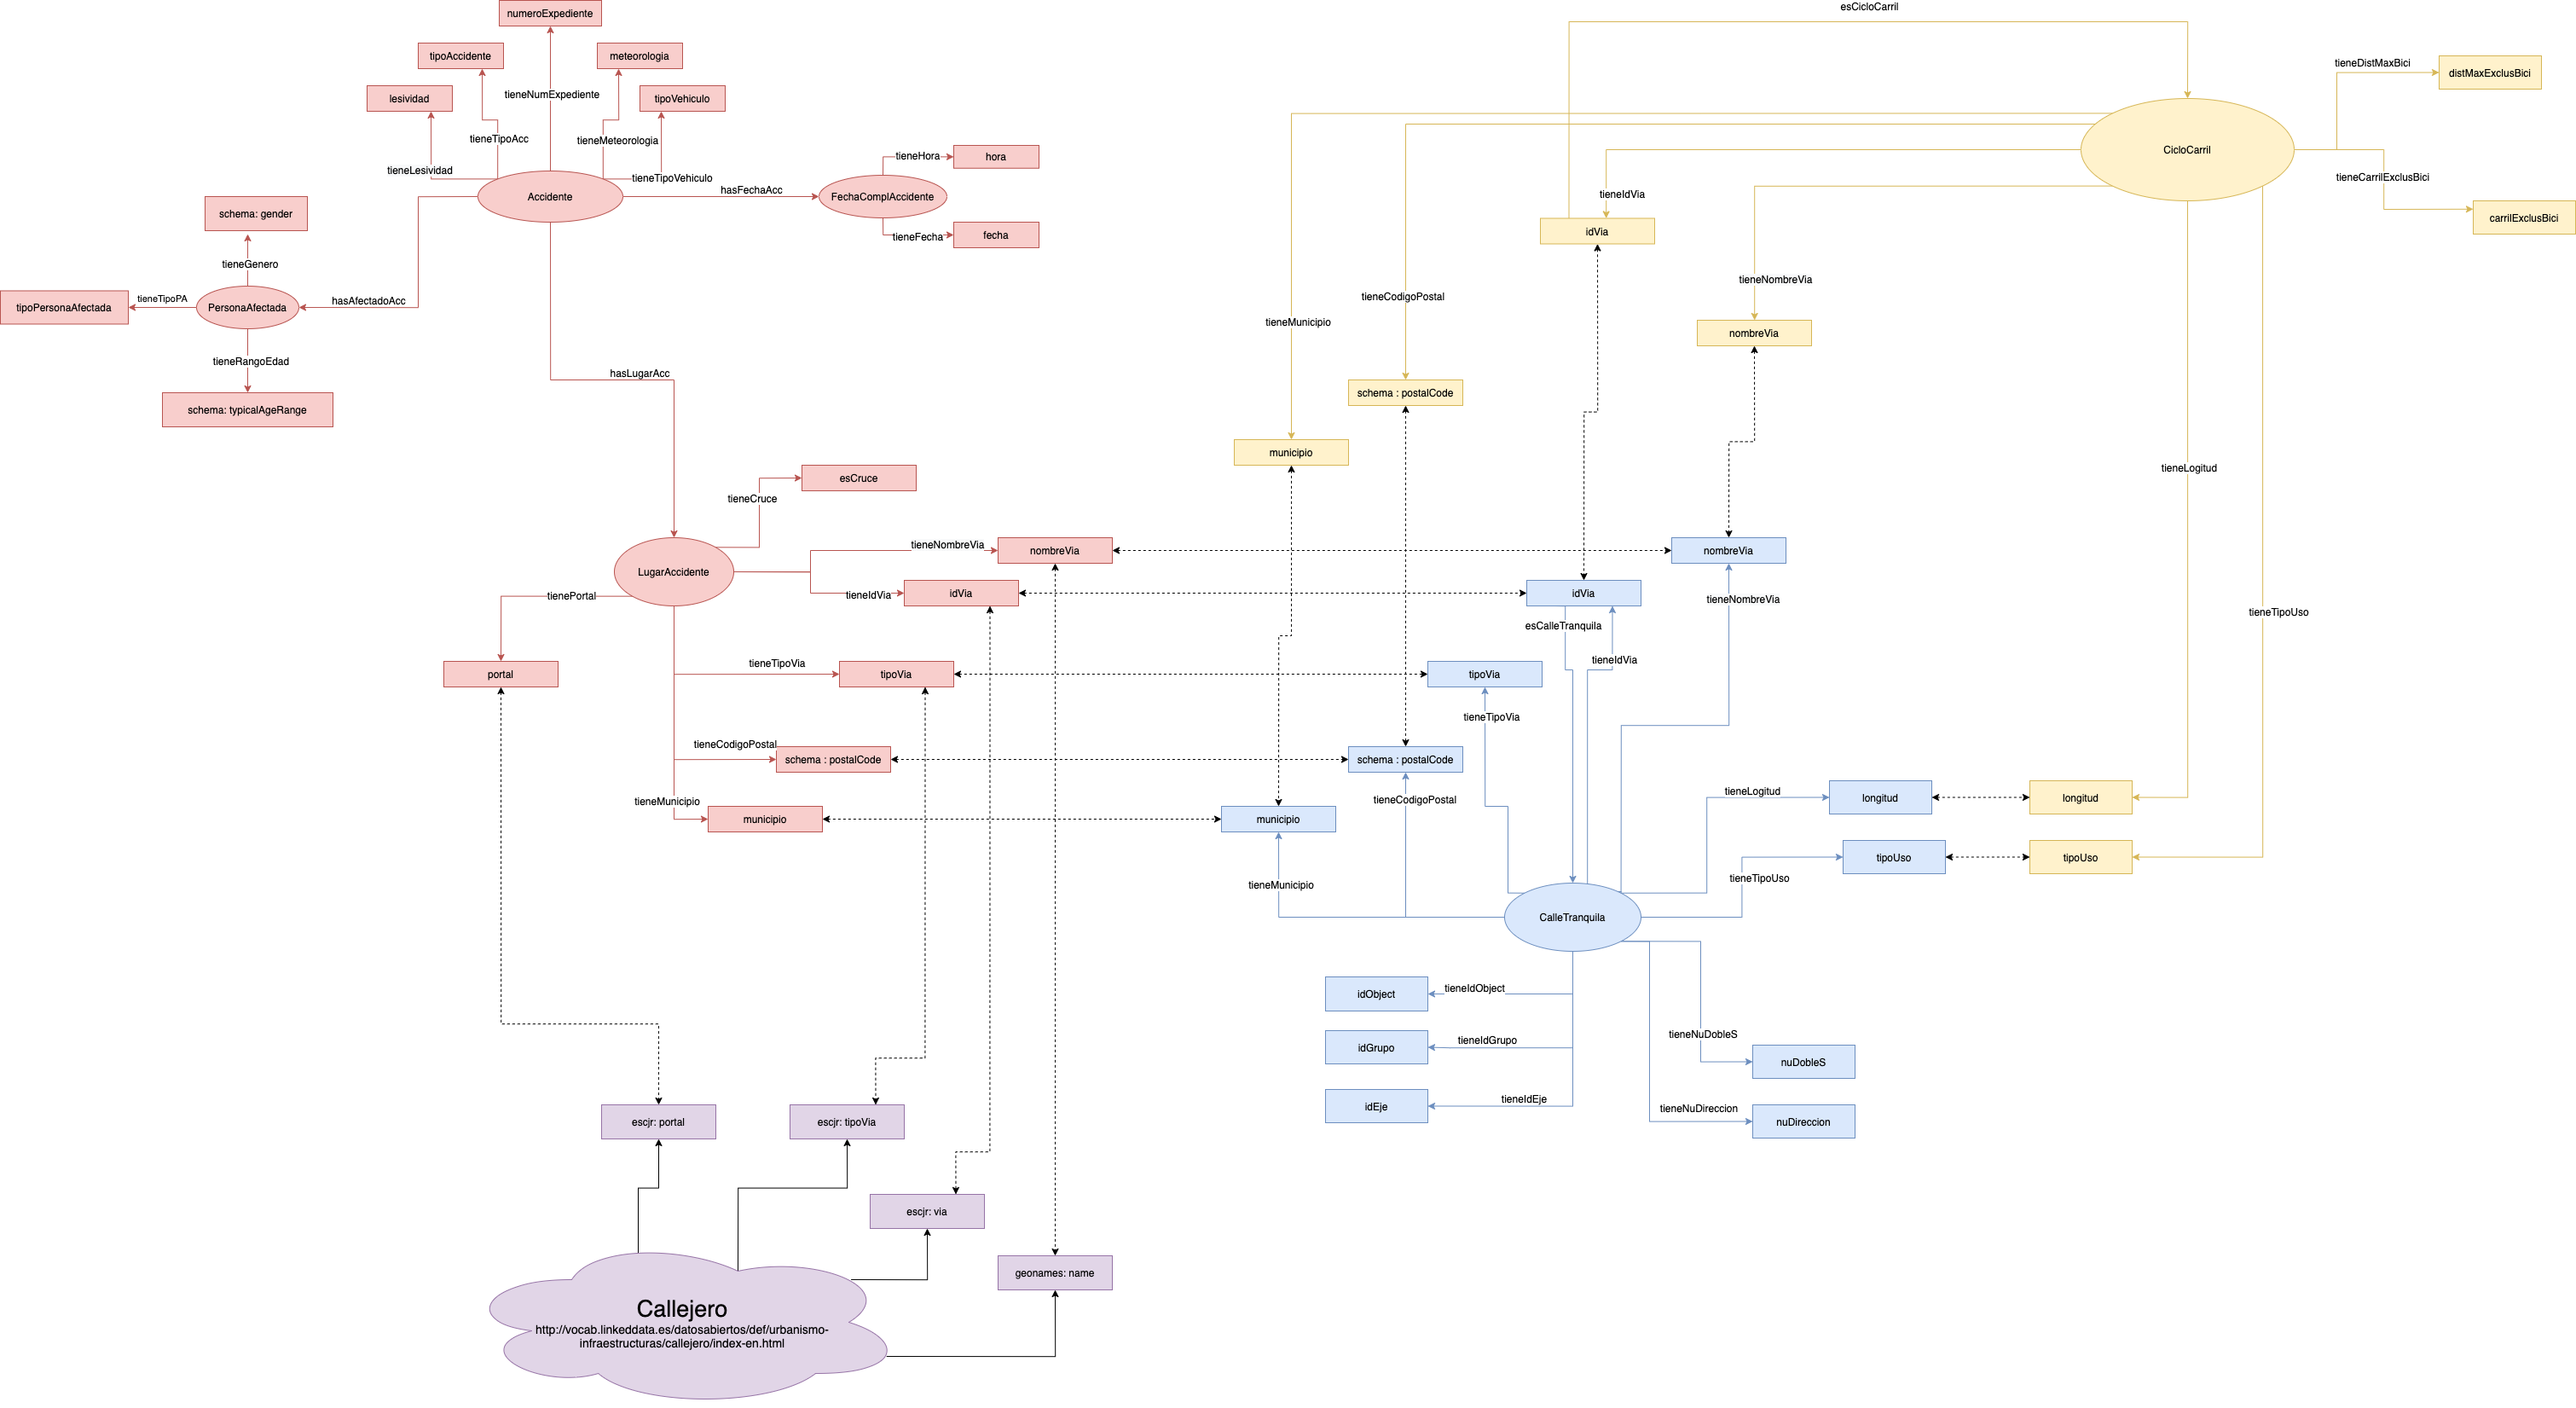
\includegraphics[angle=90, width=0.8\textwidth]{images/diagramaAppTotal.png} 
  \\
  \caption{Diagrama de los datos enlazados en la Aplicación}
  \label{fig:esquemaTotalVocab}
\end{figure}


%%---------------------------------------------------------